\documentclass[UTF8,10pt]{ctexart}

\usepackage{multicol}
\usepackage{geometry}
\usepackage{fancyhdr}
\usepackage{graphicx}
\usepackage{authblk}
\usepackage{enumerate}
\usepackage{booktabs}
\usepackage{amsmath}
\usepackage{pythonhighlight}

\setlength\columnsep{0.6cm}
\geometry{left=1.2cm,right=1.2cm,top=2.5cm,bottom=1.8cm}
\title{\vspace{-2cm}HPC101\ 实验4\quad 实验报告}
\author[ ]{张云轩*\quad 3200105087}
%\affil[ ]{3200105087}
\affil[*]{信息与电子工程学院\quad 信息工程}
\affil[*]{竺可桢学院\quad 工程教育高级班}

\date{\today}

\pagestyle{fancy}
%清除原页眉页脚样式
\fancyhf{} 
%R:页面右边;O:奇数页;\leftmark:表示“一级标题”
\fancyhead[RO]{\leftmark}
%L:页面左边;E:偶数页;\rightmark:表示“二级标题”
\fancyhead[LE]{\rightmark}
%C:页面中间
\fancyhead[CO, CE]{HPC101\ 实验4\quad 实验报告}
%同上,但是不同位置放置不同信息
\fancyhead[LO, RE]{}
% 设置页脚,页眉的位置上也可以放置页码
\fancyfoot[RO, LE]{\thepage}
\fancyfoot[LO, RE]{}
% 设置页眉页脚横线及样式
%页眉线宽,设为0可以去页眉线
\renewcommand{\headrulewidth}{0.1mm} 
%页脚线宽,设为0可以去页眉线
\renewcommand{\footrulewidth}{0mm} 

\begin{document}

\maketitle

\section{实验任务与要求}
\begin{enumerate}[1]
    \item 对于$N$阶方阵$A$、$B$和给定的自然数$n$,计算矩阵连积
            \begin{equation}
                \prod_{k = 0}^{n} (A+kB)=A(A+B)(A+2B)...(A+nB)  
            \end{equation}
            其中矩阵$A$、$B$为随机生成的signed int 32矩阵。出于方便起见无需考虑溢出。
    \item 使用每秒计算量(Operations Per Second,Ops)来评价程序性能,计算⽅法如下:
        \begin{equation}
            Ops=\frac{n}{T}C 
        \end{equation}
        其中$C=10001^3+2·10001^2$为常量。
    \item 加速GEMM(通用矩阵乘法)计算
    \item 测试加速算法的正确性和速度
    \item 提交代码和简要的思路
\end{enumerate}

\section{实验环境}
4节点集群服务器,单节点配置如下:
\paragraph{CPU} Intel(R) Xeon(R) CPU E5-2670 v3 @ 2.30GHz x48
\paragraph{Memory} 126GB
\paragraph{Network} Intel Corporation I350 Gigabit Network Connection Ethernet controller

\section{实验原理}
\subsection{程序访存局部性}
程序访存局部性指的是应用程序在访问内存的时候,倾向于访问内存中较为靠近的连续的值。

一般来说,程序的局部性分为两种形式,一种是时间局部性,另一种是空间局部性。时间局部性指的是,程序在运行时,最近刚刚被引用过的一个内存位置容易再次被引用,比如在调取一个函数的时候,前不久才调取过的本地参数容易再度被调取使用。空间局部性指的是,最近引用过的内存位置以及其周边的内存位置容易再次被使用。空间局部性比较常见于循环中,比如在一个数列中,如果第$n$个元素在上一个循环中使用,则本次循环中极有可能会使用第$n+1$个元素。

局部性是出现在计算机系统中的一种可预测行为。系统的这种强访问局部性,可以被用来在处理器内核的指令流水线中进行性能优化,如缓存,内存预读取以及分支预测。

\subsection{计算机层次存储结构}
存储层次是在计算机体系结构下存储系统层次结构的排列顺序。每一层于下一层相比都拥有较高的速度和较低延迟性,以及较小的容量。

\begin{center}
    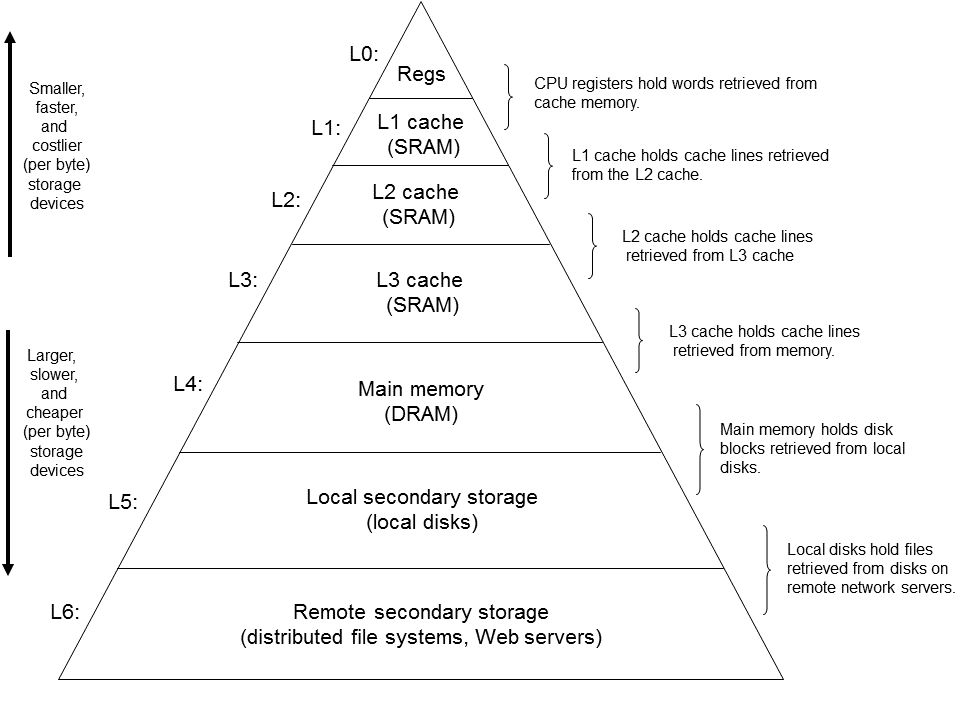
\includegraphics[scale=0.42]{img/1.jpg}
\end{center}

层次存储的设计核心目的就是要充分利用程序的局部性,如将最常访问的数据放置在较高的层级来保证访问速度;再比如按照顺序访问能够使得每次取来的整块数据都能够被利用,也使得预取的数据是有效的;如果你的内存充足,你甚至可以将硬盘上的数据提前拷贝到内存,来避免硬盘I/O带来的开销,等等。

因此,充分优化一个程序的局部性,能够使得其充分利用现代计算机硬件上各种加速设计,提高其运行效率。

\subsection{计算并行化}
计算并行化的前提是并行化的计算任务之间不存在逻辑先后上的相互依赖,彼此独立,计算的顺序并不影响结果的正确性。矩阵乘法中,结果矩阵中不同元素。或者不同分块间彼此独立,因此适用并行化。

\subsubsection{SIMD}
SIMD是一种数据并行技术,它通过提供支持向量运算的指令,同时对一组数据执行相同的计算,从而实现空间上的并行,进而提高程序的并行度和吞吐量。当程序中出现大量完全一致的运算需要对一批数据进行处理时,可以考虑使用SIMD对其进行并行。

\subsubsection{指令级并行}
现代处理器一般都会使用流水线技术来同时执行多条指令的不同阶段,从而实现指令间的并行。

\subsubsection{线程级并行}
在现代计算机中,有多个物理核心,而线程作为调度的最小单位只能在一个核心上执行,因此需要开启多个线程来充分利用每一个核心。线程具有内存共享的特点,这意味着线程间的通信开销会小不少。因此在单机上往往采用多线程的并行模型。

\subsubsection{进程级并行}
对于分布式的计算来说,仅仅使用线程并行已经不够了。需要在每个节点上开启不同的进程,来激发更多的并行能力。由于进程间的内存并不共享,需要手动维护进程间通信来进行数据的分享。

\section{实验过程}
\subsection{Baseline测试(单线程)}
Baseline中已经对naive的矩阵乘法计算作了一定的优化,例如,将右矩阵转置以提升访存局部性,提高寄存器命中率;添加了openMP的编译器制导语句实现多线程并行。首先测试不开启openMP的单线程性能。
\begin{python}
编译命令:g++ -o gemm hw_baseline.cpp -mcmodel=medium -O -march=native
\end{python}
\begin{python}
Performance : 1.645952 Gops
Validation passed.
\end{python}

\subsection{Baseline测试(openMP)}
在编译选项内使用-fopenmp选项开启openMP支持:
\begin{python}
编译命令:g++ -o gemm hw_baseline.cpp -mcmodel=medium -fopenmp -O -march=native
\end{python}
\begin{python}
Performance : 20.790923 Gops
Validation passed.
\end{python}
约获得了12.7倍的速度提升。本机(SLM)共有16核32线程,线程间通信和线程调度损失了一定的性能。

\subsection{一次计算4$\times $8个元素,在计算中使用寄存器,并使用间接寻址}
一次计算4x8个元素是为向量化做准备。

在baseline的计算中,每次标量乘法计算的结果都会立即累加到结果内存$C_{ij}$上,这将导致频繁的内存访问。因此,我们创建临时结果寄存器,每次标量乘法的结果累加到寄存器上,所有计算结束后再存储到内存中的$C_{ij}$中。

直接寻址是指类似于B[len*i+j]的寻址方式,指针B指向二维矩阵的左上角坐标,每次寻址都要先偏移i行,然后偏移j列。行偏移将在每次寻址中都引入一次乘法运算。乘法运算耗费的时间比加法多得多。鉴于每次使用的数据都位于同一行,因此考虑使用一个指针记录行首地址,之后每次寻址只需要在这个指针基础上进行列的偏移,这样就只有加法运算了,将加快计算速度。具体实现见代码注释。

\begin{python}
// main()
#pragma omp parallel for
for (int i=0; i<N; i+=4)
    for (int j=0; j<N; j+=4)
        calc_4x8(&matC2[i*N+j], &matC[i*N], &matA[j*N], N);

// calc_4x8()
void calc_4x4(int *result, int *A, int *B, int len)
{
    // 创建临时存储结果的寄存器
    register int c00_reg=0, c01_reg=0, c02_reg=0, c03_reg=0, c04_reg=0, c05_reg=0, c06_reg=0, c07_reg=0;
    register int c10_reg=0, c11_reg=0, c12_reg=0, c13_reg=0, c14_reg=0, c15_reg=0, c16_reg=0, c17_reg=0;
    register int c20_reg=0, c21_reg=0, c22_reg=0, c23_reg=0, c24_reg=0, c25_reg=0, c26_reg=0, c27_reg=0;
    register int c30_reg=0, c31_reg=0, c32_reg=0, c33_reg=0, c34_reg=0, c35_reg=0, c36_reg=0, c37_reg=0;

    // 创建指针变量指向每一行的行首。这里右矩阵B转置过,因此并不是按列读取
    int *b0_ptr=&B[0];
    int *b1_ptr=&B[len];
    int *b2_ptr=&B[2*len];
    ... // 重复不表
    int *b3_ptr=&B[7*len];


    int *a0_ptr=&A[0];
    int *a1_ptr=&A[len];
    int *a2_ptr=&A[2*len];
    ... // 重复不表
    int *a3_ptr=&A[7*len];

    // 因为是4x4的计算,因此A和B中的每个元素将被访问四次。使用寄存器存储这些元素可以进一步减少访存次数
    register int a0_reg, a1_reg, a2_reg, a3_reg;
    register int b0_reg, b1_reg, b2_reg, b3_reg, b4_reg, b5_reg, b6_reg, b7_reg;

    for(int i=0; i<len; i++)
    {   
        // 将乘法+加法运算组成的直接寻址转化为了只有自增(加法)运算的间接寻址
        a0_reg=*a0_ptr++;
        ... // 重复不表
        a3_reg=*a3_ptr++;

        b0_reg=*b0_ptr++;
        ... // 重复不表
        b3_reg=*b7_ptr++;

        c00_reg+=a0_reg*b0_reg;
        c01_reg+=a0_reg*b1_reg;
        c02_reg+=a0_reg*b2_reg;
        c03_reg+=a0_reg*b3_reg;
        ... // 重复不表
        c33_reg+=a3_reg*b7_reg;
    }

    // 全部计算结束后,再将寄存器中的结果写入内存中,只访存一次
    result[0]=c00_reg;
    result[1]=c01_reg;
    result[2]=c02_reg;
    result[3]=c03_reg;
    ... // 重复不表
    result[3*len+7]=c37_reg;

    return;
}
\end{python}
\begin{python}
编译命令:g++ -o gemm hw_4x8_reg.cpp -mcmodel=medium -fopenmp -O -march=native
\end{python}
\begin{python}
Performance : 26.117555 Gops
Validation passed.
\end{python}

\subsection{分块}
将矩阵的计算分为block\_m$\times $block\_n的区域来计算。在一般的矩阵乘法计算中,由于右矩阵$B$是行主序存储但是按列读取的,因此$B$矩阵的每一次读取都是不连续的,当矩阵规模超过一定程度时,就会导致cache命中失败。分块操作可以每次计算都使用$B$的一行,提高cache命中率。然而由于本例中,右矩阵$B$是转置过(列主序存储)的,对$B$的按列读取都是内存连续的,因此分块操作恐怕无法取得显著的效果,甚至会降低性能。
\begin{python}
// main()
const int block_m=128;
const int block_k=256;
#pragma omp parallel for
for(int i=0; i<N; i+=block_m)
    for(int j=0; j<N; j+=block_k)
        calc_block(block_m, N, block_k, &matC2[i*N+j], &matC[i*N], &matA[j*N]);

// calc_block()
void calc_block(const int block_m, const int block_n, const int block_k,
                int *result, int *A, int *B)
{
    for(int i=0; i<block_m; i+=4)
        for(int j=0; j<block_k; j+=8)
            calc_4x8(&result[i*block_n+j], &A[i*block_n], &B[j*block_n], block_n);
}
\end{python}
\begin{python}
编译命令:g++ -o gemm hw_4x8_reg_blocking.cpp -mcmodel=medium -fopenmp -O -march=native
\end{python}
\begin{python}
Performance : 22.532564 Gops
Validation passed.
\end{python}
不出所料,性能降低了。因此,在条件允许的时候,事先对右矩阵转置处理能获得比分块更好的性能。关于分块与转置的比较深入讨论,请见结论章节。

\subsection{SIMD向量化}
4.2节中的一次计算$4\times 8$个元素,是为了实现向量化。
\subsubsection{手动SIMD向量化}
\begin{python}
    void calc_4x8_AVX(int *result, int *A, int *B, int len)
{
    // 创建向量寄存器
    __m256i vec_a0, vec_a1, vec_a2, vec_a3;
    __m256i vec_c0, vec_c1, vec_c2, vec_c3;
    __m256i vec_b;
    // 创建中间结果寄存器
    __m256i vec_tmp0, vec_tmp1, vec_tmp2, vec_tmp3;

    // 用0填充累加寄存器
    vec_c0=_mm256_set1_epi32(0);
    ... // 重复不表
    vec_c3=_mm256_set1_epi32(0);

    // 相对地址指针
    int *a0_ptr=&A[0];
    ... // 重复不表
    int *a3_ptr=&A[3*len];

    for(int i=0; i<len; i++)
    {
        //将数据从内存读入向量寄存器
        vec_b=_mm256_load_si256(reinterpret_cast<__m256i const*>(B+i*len));

        vec_a0=_mm256_set1_epi32(*a0_ptr++);
        ... // 重复不表
        vec_a3=_mm256_set1_epi32(*a3_ptr++);
        
        // 向量乘
        vec_tmp0=_mm256_mullo_epi32(vec_a0, vec_b);
        ... // 重复不表
        vec_tmp3=_mm256_mullo_epi32(vec_a3, vec_b);
        // 向量加
        vec_c0=_mm256_add_epi32(vec_c0, vec_tmp0);
        ... // 重复不表
        vec_c3=_mm256_add_epi32(vec_c3, vec_tmp0);
    }

    // 将向量寄存器中的结果写回内存
    _mm256_store_si256(reinterpret_cast<__m256i *>(result), vec_c0);
    ... // 重复不表
    _mm256_store_si256(reinterpret_cast<__m256i *>(result+3*len), vec_c3);
}
\end{python}
在编译选项中添加了-mavx和-mavx2以支持向量化函数接口。
\begin{python}
编译命令:g++ -o gemm hw_4x8_AVX.cpp -mcmodel=medium -fopenmp -O -march=native -mavx -mavx2
\end{python}
\begin{python}
Performance : 54.770838 Gops
Validation passed.
\end{python}
获得了约2倍有余的性能提升。之所以没有获得8倍的理论性能提升,是因为将数据读入和卸出向量寄存器要花费额外的时间。

\subsubsection{编译器自动向量化}
手动向量化的粒度往往不及编译器自动向量化。在编译选项中加入-O3选项以开启编译器自动向量化;加入-mavx2选项指示编译器使用AVX2指令集(不然默认会使用SSE3指令集,性能不及AVX2);加入-fopt-info-vec-optimized选项查看被编译器自动向量化的语句。
\begin{python}
编译命令:g++ -o gemm hw_4x8_reg.cpp -mcmodel=medium -fopenmp -O3 -fopt-info-vec-optimized -march=native -mavx2
\end{python}
\begin{python}
hw_4x8_reg.cpp:137:23: note: loop vectorized
hw_4x8_reg.cpp:137:23: note: loop versioned for vectorization because of possible aliasing
...
Performance : 111.438199 Gops
Validation passed.
\end{python}
O3编译选项不仅将手动实现向量化的循环自动向量化,也将其他一些没有手动向量化的区域实现了自动向量化;除此之外,其优化器还在其他区域优化了代码速度。综合来看,获得了手动SIMD两倍的性能,未向量化代码4倍的性能。

\subsection{进程级并行}
为了使用集群服务器进一步提升程序并行度,考虑使用MPI框架实现进程级并行。基于集群中有四台节点,设计了程序的并行通信结构。具体的计算流程请见流程图。

\begin{center}
    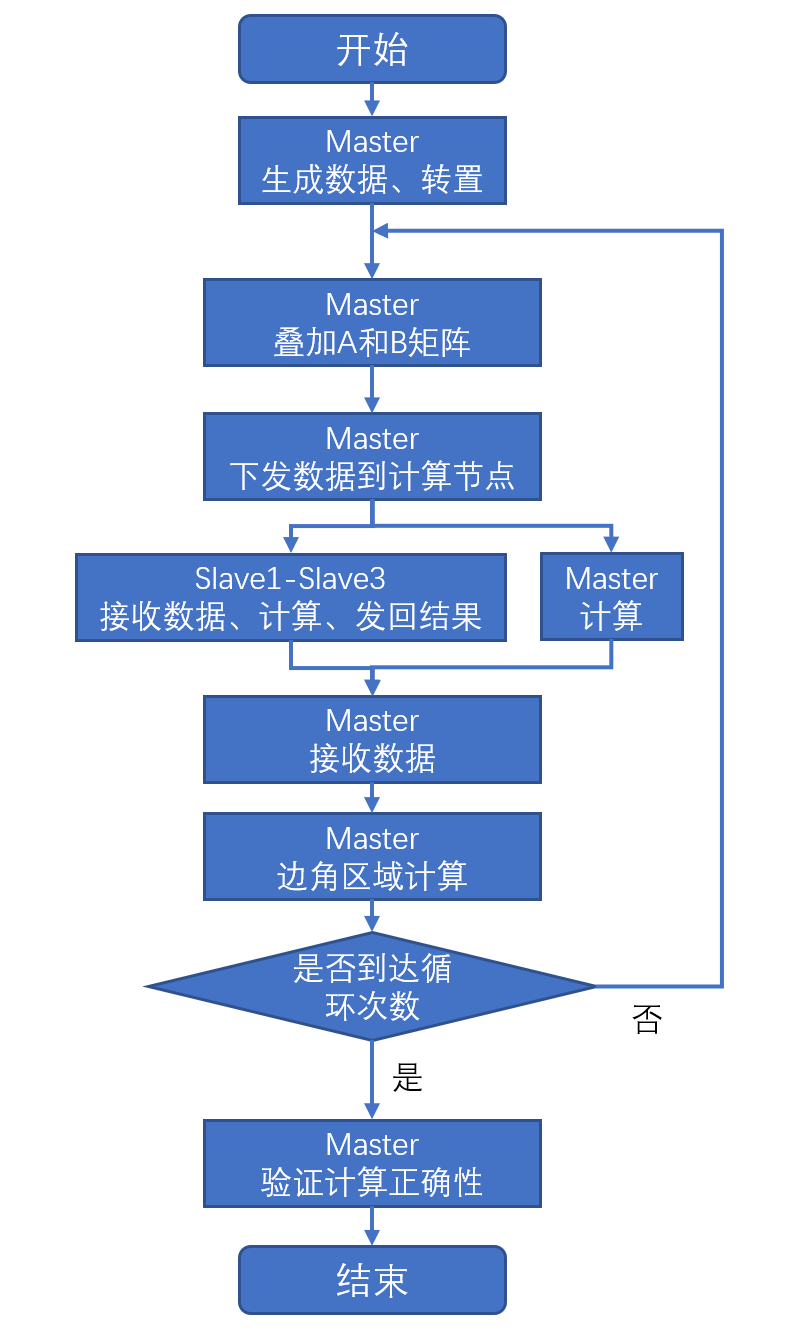
\includegraphics[scale=0.6]{img/2.PNG}
\end{center}

0号节点充当master节点(主节点),负责生成数据、分发数据到计算节点、收集计算节点发回的计算结果和检验计算结果正确性。由于评判程序性能的计时点没有记录数据生成的时间(实际上,这将占据程序运行的大部分时间!),因此没有考虑将数据的生成进程级并行化,而只是在一个节点上进行。

1-3号节点充当slave1-slave3节点(计算节点),负责接收主节点发送来的数据,计算,并将计算结果发回给主节点。

在slave节点工作过程中,主节点在等待数据发回,是空闲的。因此考虑将主节点作为slave0计算节点在等待数据发回的过程中也参与计算工作。即0号节点充当master和slave0两角。

基于以上架构,很容易想到将结果矩阵的计算划分为四块,分发到每个计算节点计算。然而,对于边长非4的倍数的矩阵,上述实现并不能计算(因为每次要计算4x4的块)。为了实现能够计算任意形状的矩阵,我们考虑将矩阵划分为尽可能大的四个边长为4的整数倍的方阵,下发到计算节点计算,主节点随后使用逐个元素计算的naive的方法计算剩下的不规则区域的结果。

由流程图分析,master节点的数据下发、数据接收和边角区域计算是比slave节点多出来的工作。当master节点做这些工作的时候,slave节点是空闲的。因此,我们考虑使用异步通信,在master节点进行下发和回收数据的通信的同时进行作为slave0节点的计算和边角计算的工作,达到掩盖访存延时的目的。具体代码实现见附件mpi\_async.cpp。
\begin{python}
编译命令:mpiicc -o gemm_mpi mpi_async.cpp -mcmodel=medium -fopenmp -Ofast -march=native -mavx2
\end{python}
\begin{python}
Performance : 395.925700 Gops
Validation passed.
\end{python}
实现了3.53倍的加速。投入了4倍的计算资源,获得了这样的加速效果是比较理想的。

\section{结论与进一步讨论}
\subsection{结论}
本实验使用分块、SIMD向量化、寄存器优化、openMP线程级并行化和MPI进程级并行化等技术,加速了GEMM通用矩阵乘法计算。最终,相对baseline(1.646Gops),获得了240.5倍的加速比(395.926Gops)。

\subsection{进一步讨论}
在实验过程中,我们发现在右矩阵转置为列主序存储模式后,使用分块操作会降低性能。这是因为右矩阵转置后,对其按列访问在内存上是连续的,如果这时候再分块,将导致块内每次的按列读取是连续的,但是下一列的读取是不连续的。这虽然减少了cache miss的频率,但总归是有;然而转置操作则完全杜绝了cache miss,最大限度地利用了寄存器加速。即在这个实验的例子中,右矩阵转置可以获得比不转置而分块更高的性能。

我们测试了不使用转置操作的baseline的性能,结果如下:
\begin{python}
编译命令:g++ -o gemm_baseline hw_baseline.cpp -mcmodel=medium -fopenmp -O -march=native
\end{python}
\begin{python}
Performance : 3.733295 Gops
Validation passed.
\end{python}
可见,与使用了转置预处理的baseline(20.791Gops)相比,未转置预处理的程序速度降低到了$1/6$左右,转置带来的加速效果十分明显。

我在Lab3的cuda GEMM计算中也尝试过转置右矩阵的操作,当时基于的考量也是内存连续性。然而,在cuda中,转置操作使得速度变慢了。猜测原因是在cuda编程中,由于核函数数以百万计,因此访存性能瓶颈主要在访存带宽而不是访存延迟上。转置后使得有多个核函数同时访问内存中的相同区域,造成带宽阻塞。而在CPU GEMM计算中带宽是足够的,影响速度的因素主要是访存延时。因此尽可能地减少访存次数将带来大幅度的速度提升。

\end{document}